\subsection{Historical review}

The early developments that led to the original MPM started with the \textbf{Particle-In-Cell} method (PIC) formulated for fluid dynamics problems \cite{PIC}. The novelty brought by PIC was the representation of a fluid by a collection of moving particles inside a background control volume subdivided into cells. Every single particle is given a constant mass and a position which is updated based on the velocity field resulting from the solution of linear momentum balance equation on the fixed background mesh. On the other hand, velocity, energy and pressure are stored at cells during the whole computation ($C^0$ approximation). A \textit{convective phase}, which consists in a weighting procedure, must be followed when a particle leaves a cell and enters a new one \cite{PIC}. Thus, the PIC enables the merging of Lagrangian and Eulerian techniques since the moving particles with ascribed masses enables the simulation of problems involving several highly deformed fluids without mesh distortion.

In spite of the good results provided by the PIC, the numerical diffusion it suffers from has been addressed by two different ways. First the method has been extended to a \textit{fully Lagrangian} approach \cite{McCrory_FLIP} by storing not only mass and position but all the fields at particles. Next, a new projection procedure has been proposed between the grid and the particles in order to reach second-order accuracy in space of the convective phase \cite{PIC_Nishiguchi}. The merging of those two improvements yielded the so-called \textbf{FLuid Implicit Particle} method (FLIP) \cite{FLIP}. In this new PIC formulation, every quantities are stored at particles so that the grid is only used for solving balance equations and hence provides an adaptive feature to the numerical scheme. The projection of fields from Lagrangian particles to the Eulerian mesh is made as in PIC while the backward mapping models the \textit{collisional} behavior of the fluid and leads to a double definition of the velocity. Indeed, the linear momentum resulting from the solution of balance equations on the grid is used to update the position of particles, whereas the change of linear momentum is used to update their velocity \cite{Mass_Flip}. This procedure yields a time derivative of particles displacement that is different from their velocity which, although it introduces oscillations in the vicinity of discontinuities, provides better results in terms of numerical diffusion \cite{Mass_Flip}.






\subsection{Derivation of the mpm}
\subsubsection{MPM discrete equations}
\subsubsection{Solution scheme summary}
\subsection{Shortcomings}
\begin{figure}[h!]
  \centering
  {\definecolor{Purple}{RGB}{120,28,129}
\definecolor{Blue}{RGB}{63,96,174}
\definecolor{Duck}{RGB}{83,158,182}
\definecolor{Green}{RGB}{109,179,136}
\definecolor{Yellow}{RGB}{202,184,67}
\definecolor{Orange}{RGB}{231,133,50}
\definecolor{Red}{RGB}{217,33,32}
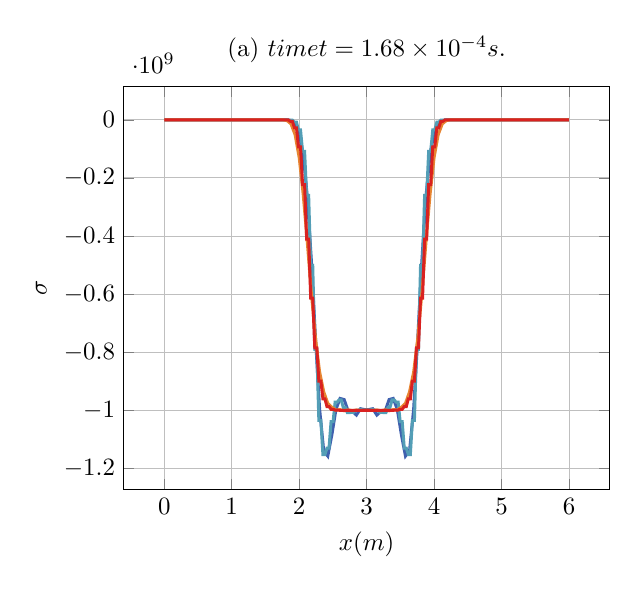
\begin{tikzpicture}[scale=0.9]
\begin{axis}[xlabel=$x (m)$,ylabel=$\sigma$,ymajorgrids=true,xmajorgrids=true,title={(a) $time t= 1.68\times 10^{-4}s.$}]
\addplot[Blue,very thick] coordinates {(0.0,0.0) (0.0606060606061,0.0) (0.121212121212,0.0) (0.181818181818,0.0) (0.242424242424,-9.52481580298e-08) (0.30303030303,1.9049631606e-07) (0.363636363636,0.0) (0.424242424242,9.52481580298e-08) (0.484848484848,-9.52481580298e-08) (0.545454545455,-9.52481580298e-08) (0.606060606061,0.0) (0.666666666667,0.0) (0.727272727273,0.0) (0.787878787879,0.0) (0.848484848485,0.0) (0.909090909091,0.0) (0.969696969697,0.0) (1.0303030303,0.0) (1.09090909091,0.0) (1.15151515152,0.0) (1.21212121212,0.0) (1.27272727273,0.0) (1.33333333333,0.0) (1.39393939394,0.0) (1.45454545455,0.0) (1.51515151515,0.0) (1.57575757576,0.0) (1.63636363636,0.0) (1.69696969697,0.0) (1.75757575758,0.0) (1.81818181818,-290909.240339) (1.87878787879,-2464283.65777) (1.93939393939,-12475539.1386) (2.0,-44052889.5401) (2.06060606061,-120831137.543) (2.12121212121,-266470659.018) (2.18181818182,-488473559.025) (2.24242424242,-753632810.849) (2.30303030303,-995980052.752) (2.36363636364,-1139088359.69) (2.42424242424,-1157623631.23) (2.48484848485,-1084032532.28) (2.54545454545,-996796489.138) (2.60606060606,-959183611.366) (2.66666666667,-963021938.112) (2.72727272727,-1003176408.24) (2.78787878788,-1003828199.65) (2.84848484848,-1016372455.45) (2.90909090909,-994660368.744) (2.9696969697,-997544165.333) (3.0303030303,-997544165.333) (3.09090909091,-994660368.744) (3.15151515152,-1016372455.45) (3.21212121212,-1003828199.65) (3.27272727273,-1003176408.24) (3.33333333333,-963021938.112) (3.39393939394,-959183611.366) (3.45454545455,-996796489.138) (3.51515151515,-1084032532.28) (3.57575757576,-1157623631.23) (3.63636363636,-1139088359.69) (3.69696969697,-995980052.752) (3.75757575758,-753632810.849) (3.81818181818,-488473559.025) (3.87878787879,-266470659.018) (3.93939393939,-120831137.543) (4.0,-44052889.5401) (4.06060606061,-12475539.1386) (4.12121212121,-2464283.65777) (4.18181818182,-290909.240339) (4.24242424242,0.0) (4.30303030303,0.0) (4.36363636364,0.0) (4.42424242424,0.0) (4.48484848485,0.0) (4.54545454545,0.0) (4.60606060606,0.0) (4.66666666667,0.0) (4.72727272727,0.0) (4.78787878788,0.0) (4.84848484848,0.0) (4.90909090909,0.0) (4.9696969697,0.0) (5.0303030303,0.0) (5.09090909091,0.0) (5.15151515152,0.0) (5.21212121212,0.0) (5.27272727273,0.0) (5.33333333333,0.0) (5.39393939394,0.0) (5.45454545455,0.0) (5.51515151515,0.0) (5.57575757576,0.0) (5.63636363636,0.0) (5.69696969697,0.0) (5.75757575758,0.0) (5.81818181818,0.0) (5.87878787879,0.0) (5.93939393939,0.0) (6.0,0.0) };
\addplot[Duck,very thick] coordinates {(0.0,9.47695240698e-08) (0.0301507537688,9.47695240698e-08) (0.0603015075377,0.0) (0.0904522613065,0.0) (0.120603015075,0.0) (0.150753768844,0.0) (0.180904522613,-9.47695240698e-08) (0.211055276382,-9.47695240698e-08) (0.241206030151,-9.47695240698e-08) (0.27135678392,-9.47695240698e-08) (0.301507537688,3.85185988877e-23) (0.331658291457,3.85185988877e-23) (0.361809045226,-1.8953904814e-07) (0.391959798995,-1.8953904814e-07) (0.422110552764,-1.15555796663e-22) (0.452261306533,-1.15555796663e-22) (0.482412060302,-3.79078096279e-07) (0.51256281407,-3.79078096279e-07) (0.542713567839,-9.47695240698e-08) (0.572864321608,-9.47695240698e-08) (0.603015075377,-2.84308572209e-07) (0.633165829146,-2.84308572209e-07) (0.663316582915,-1.8953904814e-07) (0.693467336683,-1.8953904814e-07) (0.723618090452,-5.68617144419e-07) (0.753768844221,-5.68617144419e-07) (0.78391959799,-2.84308572209e-07) (0.814070351759,-2.84308572209e-07) (0.844221105528,0.0) (0.874371859296,0.0) (0.904522613065,3.79078096279e-07) (0.934673366834,3.79078096279e-07) (0.964824120603,1.92592994439e-23) (0.994974874372,1.92592994439e-23) (1.02512562814,-3.85185988877e-23) (1.05527638191,-3.85185988877e-23) (1.08542713568,-1.8953904814e-07) (1.11557788945,-1.8953904814e-07) (1.14572864322,3.85185988877e-23) (1.17587939698,3.85185988877e-23) (1.20603015075,1.92592994439e-23) (1.23618090452,1.92592994439e-23) (1.26633165829,-9.47695240698e-08) (1.29648241206,-9.47695240698e-08) (1.32663316583,0.0) (1.3567839196,0.0) (1.38693467337,1.8953904814e-07) (1.41708542714,1.8953904814e-07) (1.4472361809,-9.47695240698e-08) (1.47738693467,-9.47695240698e-08) (1.50753768844,-1.8953904814e-07) (1.53768844221,-1.8953904814e-07) (1.56783919598,-3.79078096279e-07) (1.59798994975,-3.79078096279e-07) (1.62814070352,7.70371977755e-23) (1.65829145729,7.70371977755e-23) (1.68844221106,-3.79078096279e-07) (1.71859296482,-3.79078096279e-07) (1.74874371859,-4.73847620349e-07) (1.77889447236,-4.73847620349e-07) (1.80904522613,-101217.236572) (1.8391959799,-101217.236572) (1.86934673367,-1285752.16656) (1.89949748744,-1285752.16656) (1.92964824121,-8237349.40661) (1.95979899497,-8237349.40661) (1.98994974874,-34844550.3527) (2.02010050251,-34844550.3527) (2.05025125628,-108179444.374) (2.08040201005,-108179444.374) (2.11055276382,-260321704.108) (2.14070351759,-260321704.108) (2.17085427136,-501459053.925) (2.20100502513,-501459053.925) (2.23115577889,-789868700.052) (2.26130653266,-789868700.052) (2.29145728643,-1035125165.66) (2.3216080402,-1035125165.66) (2.35175879397,-1152506832.27) (2.38190954774,-1152506832.27) (2.41206030151,-1130033136.46) (2.44221105528,-1130033136.46) (2.47236180905,-1039290464.94) (2.50251256281,-1039290464.94) (2.53266331658,-971601919.03) (2.56281407035,-971601919.03) (2.59296482412,-964113746.852) (2.62311557789,-964113746.852) (2.65326633166,-989886519.992) (2.68341708543,-989886519.992) (2.7135678392,-1008174894.0) (2.74371859296,-1008174894.0) (2.77386934673,-1007128879.4) (2.8040201005,-1007128879.4) (2.83417085427,-999920598.01) (2.86432160804,-999920598.01) (2.89447236181,-997978216.511) (2.92462311558,-997978216.511) (2.95477386935,-999941855.266) (2.98492462312,-999941855.266) (3.01507537688,-999941855.266) (3.04522613065,-999941855.266) (3.07537688442,-997978216.511) (3.10552763819,-997978216.511) (3.13567839196,-999920598.01) (3.16582914573,-999920598.01) (3.1959798995,-1007128879.4) (3.22613065327,-1007128879.4) (3.25628140704,-1008174894.0) (3.2864321608,-1008174894.0) (3.31658291457,-989886519.992) (3.34673366834,-989886519.992) (3.37688442211,-964113746.852) (3.40703517588,-964113746.852) (3.43718592965,-971601919.03) (3.46733668342,-971601919.03) (3.49748743719,-1039290464.94) (3.52763819095,-1039290464.94) (3.55778894472,-1130033136.46) (3.58793969849,-1130033136.46) (3.61809045226,-1152506832.27) (3.64824120603,-1152506832.27) (3.6783919598,-1035125165.66) (3.70854271357,-1035125165.66) (3.73869346734,-789868700.052) (3.76884422111,-789868700.052) (3.79899497487,-501459053.925) (3.82914572864,-501459053.925) (3.85929648241,-260321704.108) (3.88944723618,-260321704.108) (3.91959798995,-108179444.374) (3.94974874372,-108179444.374) (3.97989949749,-34844550.3527) (4.01005025126,-34844550.3527) (4.04020100503,-8237349.40661) (4.07035175879,-8237349.40661) (4.10050251256,-1285752.16656) (4.13065326633,-1285752.16656) (4.1608040201,-101217.236572) (4.19095477387,-101217.236572) (4.22110552764,-9.47695240698e-08) (4.25125628141,-9.47695240698e-08) (4.28140703518,-9.47695240698e-08) (4.31155778894,-9.47695240698e-08) (4.34170854271,1.8953904814e-07) (4.37185929648,1.8953904814e-07) (4.40201005025,-1.15555796663e-22) (4.43216080402,-1.15555796663e-22) (4.46231155779,1.8953904814e-07) (4.49246231156,1.8953904814e-07) (4.52261306533,-9.47695240698e-08) (4.5527638191,-9.47695240698e-08) (4.58291457286,9.47695240698e-08) (4.61306532663,9.47695240698e-08) (4.6432160804,2.84308572209e-07) (4.67336683417,2.84308572209e-07) (4.70351758794,-9.47695240698e-08) (4.73366834171,-9.47695240698e-08) (4.76381909548,9.47695240698e-08) (4.79396984925,9.47695240698e-08) (4.82412060302,-9.47695240698e-08) (4.85427135678,-9.47695240698e-08) (4.88442211055,3.79078096279e-07) (4.91457286432,3.79078096279e-07) (4.94472361809,9.47695240698e-08) (4.97487437186,9.47695240698e-08) (5.00502512563,-9.47695240698e-08) (5.0351758794,-9.47695240698e-08) (5.06532663317,-3.79078096279e-07) (5.09547738693,-3.79078096279e-07) (5.1256281407,-9.47695240698e-08) (5.15577889447,-9.47695240698e-08) (5.18592964824,2.84308572209e-07) (5.21608040201,2.84308572209e-07) (5.24623115578,9.47695240698e-08) (5.27638190955,9.47695240698e-08) (5.30653266332,-3.79078096279e-07) (5.33668341709,-3.79078096279e-07) (5.36683417085,-9.62964972194e-23) (5.39698492462,-9.62964972194e-23) (5.42713567839,0.0) (5.45728643216,0.0) (5.48743718593,9.47695240698e-08) (5.5175879397,9.47695240698e-08) (5.54773869347,-3.79078096279e-07) (5.57788944724,-3.79078096279e-07) (5.60804020101,-1.8953904814e-07) (5.63819095477,-1.8953904814e-07) (5.66834170854,3.85185988877e-23) (5.69849246231,3.85185988877e-23) (5.72864321608,1.8953904814e-07) (5.75879396985,1.8953904814e-07) (5.78894472362,1.8953904814e-07) (5.81909547739,1.8953904814e-07) (5.84924623116,-9.47695240698e-08) (5.87939698492,-9.47695240698e-08) (5.90954773869,-1.8953904814e-07) (5.93969849246,-1.8953904814e-07) (5.96984924623,9.47695240698e-08) (6.0,9.47695240698e-08) };
\addplot[Orange,very thick ] coordinates {(0.0,0.0) (0.0606060606061,1.92592994439e-23) (0.121212121212,2.85744474089e-07) (0.181818181818,3.80992632119e-07) (0.242424242424,4.76240790149e-07) (0.30303030303,3.80992632119e-07) (0.363636363636,1.9049631606e-07) (0.424242424242,2.85744474089e-07) (0.484848484848,0.0) (0.545454545455,-9.52481580298e-08) (0.606060606061,-9.52481580298e-08) (0.666666666667,-9.52481580298e-08) (0.727272727273,-9.52481580298e-08) (0.787878787879,-9.52481580298e-08) (0.848484848485,-9.52481580298e-08) (0.909090909091,-9.52481580298e-08) (0.969696969697,-9.52481580298e-08) (1.0303030303,-9.52481580298e-08) (1.09090909091,-9.52481580298e-08) (1.15151515152,-9.52481580298e-08) (1.21212121212,-9.52481580298e-08) (1.27272727273,-9.52481580298e-08) (1.33333333333,-9.52481580298e-08) (1.39393939394,-9.52481580298e-08) (1.45454545455,-9.52481580298e-08) (1.51515151515,-9.52481580298e-08) (1.57575757576,-9.52481580298e-08) (1.63636363636,-9.52481580298e-08) (1.69696969697,0.0) (1.75757575758,0.0) (1.81818181818,-2293510.40585) (1.87878787879,-14067645.6376) (1.93939393939,-51178965.4884) (2.0,-129583096.393) (2.06060606061,-258648404.915) (2.12121212121,-423694886.134) (2.18181818182,-600427488.416) (2.24242424242,-752616010.137) (2.30303030303,-868157986.136) (2.36363636364,-936096961.154) (2.42424242424,-976256178.588) (2.48484848485,-989436750.588) (2.54545454545,-999275981.217) (2.60606060606,-997478416.143) (2.66666666667,-1001694272.56) (2.72727272727,-998316425.19) (2.78787878788,-1001408426.26) (2.84848484848,-998924386.444) (2.90909090909,-1000673642.84) (2.9696969697,-999770565.35) (3.0303030303,-999770565.35) (3.09090909091,-1000673642.84) (3.15151515152,-998924386.444) (3.21212121212,-1001408426.26) (3.27272727273,-998316425.19) (3.33333333333,-1001694272.56) (3.39393939394,-997478416.143) (3.45454545455,-999275981.217) (3.51515151515,-989436750.588) (3.57575757576,-976256178.588) (3.63636363636,-936096961.154) (3.69696969697,-868157986.136) (3.75757575758,-752616010.137) (3.81818181818,-600427488.416) (3.87878787879,-423694886.134) (3.93939393939,-258648404.915) (4.0,-129583096.393) (4.06060606061,-51178965.4884) (4.12121212121,-14067645.6376) (4.18181818182,-2293510.40585) (4.24242424242,0.0) (4.30303030303,0.0) (4.36363636364,0.0) (4.42424242424,0.0) (4.48484848485,0.0) (4.54545454545,0.0) (4.60606060606,0.0) (4.66666666667,0.0) (4.72727272727,0.0) (4.78787878788,0.0) (4.84848484848,0.0) (4.90909090909,0.0) (4.9696969697,0.0) (5.0303030303,0.0) (5.09090909091,0.0) (5.15151515152,0.0) (5.21212121212,0.0) (5.27272727273,0.0) (5.33333333333,0.0) (5.39393939394,0.0) (5.45454545455,0.0) (5.51515151515,0.0) (5.57575757576,0.0) (5.63636363636,0.0) (5.69696969697,0.0) (5.75757575758,0.0) (5.81818181818,0.0) (5.87878787879,0.0) (5.93939393939,0.0) (6.0,0.0) };
\addplot[Red,very thick ] coordinates {(0.0,-1.92592994439e-23) (0.0301507537688,-1.92592994439e-23) (0.0603015075377,0.0) (0.0904522613065,0.0) (0.120603015075,3.79078096279e-07) (0.150753768844,3.79078096279e-07) (0.180904522613,3.79078096279e-07) (0.211055276382,3.79078096279e-07) (0.241206030151,5.68617144419e-07) (0.27135678392,5.68617144419e-07) (0.301507537688,4.73847620349e-07) (0.331658291457,4.73847620349e-07) (0.361809045226,6.63386668489e-07) (0.391959798995,6.63386668489e-07) (0.422110552764,4.73847620349e-07) (0.452261306533,4.73847620349e-07) (0.482412060302,1.8953904814e-07) (0.51256281407,1.8953904814e-07) (0.542713567839,-3.85185988877e-23) (0.572864321608,-3.85185988877e-23) (0.603015075377,0.0) (0.633165829146,0.0) (0.663316582915,-2.84308572209e-07) (0.693467336683,-2.84308572209e-07) (0.723618090452,-3.79078096279e-07) (0.753768844221,-3.79078096279e-07) (0.78391959799,-2.84308572209e-07) (0.814070351759,-2.84308572209e-07) (0.844221105528,-5.68617144419e-07) (0.874371859296,-5.68617144419e-07) (0.904522613065,-8.52925716628e-07) (0.934673366834,-8.52925716628e-07) (0.964824120603,-8.52925716628e-07) (0.994974874372,-8.52925716628e-07) (1.02512562814,-1.13723428884e-06) (1.05527638191,-1.13723428884e-06) (1.08542713568,-8.52925716628e-07) (1.11557788945,-8.52925716628e-07) (1.14572864322,-4.73847620349e-07) (1.17587939698,-4.73847620349e-07) (1.20603015075,-4.73847620349e-07) (1.23618090452,-4.73847620349e-07) (1.26633165829,-6.63386668489e-07) (1.29648241206,-6.63386668489e-07) (1.32663316583,-3.79078096279e-07) (1.3567839196,-3.79078096279e-07) (1.38693467337,-3.79078096279e-07) (1.41708542714,-3.79078096279e-07) (1.4472361809,-1.8953904814e-07) (1.47738693467,-1.8953904814e-07) (1.50753768844,-9.47695240698e-08) (1.53768844221,-9.47695240698e-08) (1.56783919598,-2.84308572209e-07) (1.59798994975,-2.84308572209e-07) (1.62814070352,-4.73847620349e-07) (1.65829145729,-4.73847620349e-07) (1.68844221106,9.47695240698e-08) (1.71859296482,9.47695240698e-08) (1.74874371859,-9.47695240698e-08) (1.77889447236,-9.47695240698e-08) (1.80904522613,-428918.453461) (1.8391959799,-428918.453461) (1.86934673367,-5033666.79954) (1.89949748744,-5033666.79954) (1.92964824121,-27410214.0671) (1.95979899497,-27410214.0671) (1.98994974874,-92954611.2088) (2.02010050251,-92954611.2088) (2.05025125628,-223143442.95) (2.08040201005,-223143442.95) (2.11055276382,-410341596.514) (2.14070351759,-410341596.514) (2.17085427136,-613519956.855) (2.20100502513,-613519956.855) (2.23115577889,-784791156.092) (2.26130653266,-784791156.092) (2.29145728643,-899163304.059) (2.3216080402,-899163304.059) (2.35175879397,-960490399.465) (2.38190954774,-960490399.465) (2.41206030151,-987121852.013) (2.44221105528,-987121852.013) (2.47236180905,-996528576.517) (2.50251256281,-996528576.517) (2.53266331658,-999232202.153) (2.56281407035,-999232202.153) (2.59296482412,-999862236.989) (2.62311557789,-999862236.989) (2.65326633166,-999980261.044) (2.68341708543,-999980261.044) (2.7135678392,-999997802.489) (2.74371859296,-999997802.489) (2.77386934673,-999999812.431) (2.8040201005,-999999812.431) (2.83417085427,-999999991.061) (2.86432160804,-999999991.061) (2.89447236181,-999999998.496) (2.92462311558,-999999998.496) (2.95477386935,-1000000000.34) (2.98492462312,-1000000000.34) (3.01507537688,-1000000000.34) (3.04522613065,-1000000000.34) (3.07537688442,-999999998.496) (3.10552763819,-999999998.496) (3.13567839196,-999999991.061) (3.16582914573,-999999991.061) (3.1959798995,-999999812.431) (3.22613065327,-999999812.431) (3.25628140704,-999997802.489) (3.2864321608,-999997802.489) (3.31658291457,-999980261.044) (3.34673366834,-999980261.044) (3.37688442211,-999862236.989) (3.40703517588,-999862236.989) (3.43718592965,-999232202.153) (3.46733668342,-999232202.153) (3.49748743719,-996528576.517) (3.52763819095,-996528576.517) (3.55778894472,-987121852.013) (3.58793969849,-987121852.013) (3.61809045226,-960490399.465) (3.64824120603,-960490399.465) (3.6783919598,-899163304.059) (3.70854271357,-899163304.059) (3.73869346734,-784791156.092) (3.76884422111,-784791156.092) (3.79899497487,-613519956.855) (3.82914572864,-613519956.855) (3.85929648241,-410341596.514) (3.88944723618,-410341596.514) (3.91959798995,-223143442.95) (3.94974874372,-223143442.95) (3.97989949749,-92954611.2088) (4.01005025126,-92954611.2088) (4.04020100503,-27410214.0671) (4.07035175879,-27410214.0671) (4.10050251256,-5033666.79954) (4.13065326633,-5033666.79954) (4.1608040201,-428918.453461) (4.19095477387,-428918.453461) (4.22110552764,6.63386668489e-07) (4.25125628141,6.63386668489e-07) (4.28140703518,5.68617144419e-07) (4.31155778894,5.68617144419e-07) (4.34170854271,4.73847620349e-07) (4.37185929648,4.73847620349e-07) (4.40201005025,5.68617144419e-07) (4.43216080402,5.68617144419e-07) (4.46231155779,5.68617144419e-07) (4.49246231156,5.68617144419e-07) (4.52261306533,5.68617144419e-07) (4.5527638191,5.68617144419e-07) (4.58291457286,6.63386668489e-07) (4.61306532663,6.63386668489e-07) (4.6432160804,6.63386668489e-07) (4.67336683417,6.63386668489e-07) (4.70351758794,6.63386668489e-07) (4.73366834171,6.63386668489e-07) (4.76381909548,2.84308572209e-07) (4.79396984925,2.84308572209e-07) (4.82412060302,-9.47695240698e-08) (4.85427135678,-9.47695240698e-08) (4.88442211055,-3.79078096279e-07) (4.91457286432,-3.79078096279e-07) (4.94472361809,-5.68617144419e-07) (4.97487437186,-5.68617144419e-07) (5.00502512563,-1.8953904814e-07) (5.0351758794,-1.8953904814e-07) (5.06532663317,1.8953904814e-07) (5.09547738693,1.8953904814e-07) (5.1256281407,1.8953904814e-07) (5.15577889447,1.8953904814e-07) (5.18592964824,1.8953904814e-07) (5.21608040201,1.8953904814e-07) (5.24623115578,9.47695240698e-08) (5.27638190955,9.47695240698e-08) (5.30653266332,1.8953904814e-07) (5.33668341709,1.8953904814e-07) (5.36683417085,-3.85185988877e-23) (5.39698492462,-3.85185988877e-23) (5.42713567839,-2.84308572209e-07) (5.45728643216,-2.84308572209e-07) (5.48743718593,-4.73847620349e-07) (5.5175879397,-4.73847620349e-07) (5.54773869347,-8.52925716628e-07) (5.57788944724,-8.52925716628e-07) (5.60804020101,-4.73847620349e-07) (5.63819095477,-4.73847620349e-07) (5.66834170854,-2.84308572209e-07) (5.69849246231,-2.84308572209e-07) (5.72864321608,-9.47695240698e-08) (5.75879396985,-9.47695240698e-08) (5.78894472362,1.8953904814e-07) (5.81909547739,1.8953904814e-07) (5.84924623116,6.63386668489e-07) (5.87939698492,6.63386668489e-07) (5.90954773869,3.79078096279e-07) (5.93969849246,3.79078096279e-07) (5.96984924623,0.0) (6.0,0.0) };
%\legend{mpm 1ppc,mpm 2ppc,modmpm 1ppc,modmpm 2ppc}
\end{axis}
\end{tikzpicture}
 \phantomsubcaption \label{subfig:mpm_diffusion_20}}
  {\definecolor{Purple}{RGB}{120,28,129}
\definecolor{Blue}{RGB}{63,96,174}
\definecolor{Duck}{RGB}{83,158,182}
\definecolor{Green}{RGB}{109,179,136}
\definecolor{Yellow}{RGB}{202,184,67}
\definecolor{Orange}{RGB}{231,133,50}
\definecolor{Red}{RGB}{217,33,32}
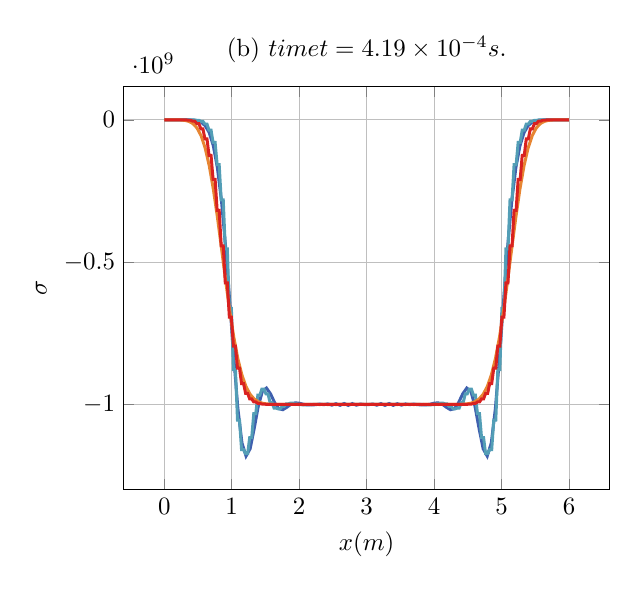
\begin{tikzpicture}[scale=0.9]
\begin{axis}[xlabel=$x (m)$,ylabel=$\sigma$,ymajorgrids=true,xmajorgrids=true,title={(b) $time t=4.19\times 10^{-4}s.$}]
\addplot[Blue,very thick] coordinates {(0.0,-1.94663032456) (0.0606060606061,-36.3841752541) (0.121212121212,-375.238546687) (0.181818181818,-2728.93329142) (0.242424242424,-15491.6755992) (0.30303030303,-72383.0822735) (0.363636363636,-287676.073247) (0.424242424242,-993977.279852) (0.484848484848,-3032319.67688) (0.545454545455,-8260134.72186) (0.606060606061,-20261581.7053) (0.666666666667,-45038635.0681) (0.727272727273,-91159838.1032) (0.787878787879,-168606730.533) (0.848484848485,-285714792.032) (0.909090909091,-444407141.455) (0.969696969697,-635335615.872) (1.0303030303,-835776800.76) (1.09090909091,-1013163065.59) (1.15151515152,-1134879131.54) (1.21212121212,-1181307983.15) (1.27272727273,-1155635730.19) (1.33333333333,-1084294024.14) (1.39393939394,-1005878929.59) (1.45454545455,-953906993.163) (1.51515151515,-942329563.046) (1.57575757576,-962785683.66) (1.63636363636,-993516383.993) (1.69696969697,-1014685599.48) (1.75757575758,-1018300742.06) (1.81818181818,-1009687906.71) (1.87878787879,-999067716.116) (1.93939393939,-994180590.642) (2.0,-995424204.967) (2.06060606061,-999165808.857) (2.12121212121,-1001723988.73) (2.18181818182,-1001348192.89) (2.24242424242,-1000885790.49) (2.30303030303,-998749472.328) (2.36363636364,-1000695729.7) (2.42424242424,-998223387.226) (2.48484848485,-1002342309.79) (2.54545454545,-997434314.666) (2.60606060606,-1003129109.15) (2.66666666667,-996584912.592) (2.72727272727,-1003333511.68) (2.78787878788,-996939459.453) (2.84848484848,-1002482461.34) (2.90909090909,-998403110.646) (2.9696969697,-1000547931.88) (3.0303030303,-1000547931.88) (3.09090909091,-998403110.646) (3.15151515152,-1002482461.34) (3.21212121212,-996939459.453) (3.27272727273,-1003333511.68) (3.33333333333,-996584912.592) (3.39393939394,-1003129109.15) (3.45454545455,-997434314.666) (3.51515151515,-1002342309.79) (3.57575757576,-998223387.226) (3.63636363636,-1000695729.7) (3.69696969697,-998749472.328) (3.75757575758,-1000885790.49) (3.81818181818,-1001348192.89) (3.87878787879,-1001723988.73) (3.93939393939,-999165808.857) (4.0,-995424204.967) (4.06060606061,-994180590.642) (4.12121212121,-999067716.116) (4.18181818182,-1009687906.71) (4.24242424242,-1018300742.06) (4.30303030303,-1014685599.48) (4.36363636364,-993516383.993) (4.42424242424,-962785683.66) (4.48484848485,-942329563.046) (4.54545454545,-953906993.163) (4.60606060606,-1005878929.59) (4.66666666667,-1084294024.14) (4.72727272727,-1155635730.19) (4.78787878788,-1181307983.15) (4.84848484848,-1134879131.54) (4.90909090909,-1013163065.59) (4.9696969697,-835776800.76) (5.0303030303,-635335615.872) (5.09090909091,-444407141.455) (5.15151515152,-285714792.032) (5.21212121212,-168606730.533) (5.27272727273,-91159838.1032) (5.33333333333,-45038635.0681) (5.39393939394,-20261581.7053) (5.45454545455,-8260134.72186) (5.51515151515,-3032319.67688) (5.57575757576,-993977.279851) (5.63636363636,-287676.073247) (5.69696969697,-72383.0822733) (5.75757575758,-15491.6755993) (5.81818181818,-2728.93329142) (5.87878787879,-375.238546687) (5.93939393939,-36.3841754446) (6.0,-1.94663032456) };
\addplot[Duck,very thick] coordinates {(0.0,-0.121116399456) (0.0301507537688,-0.121116399456) (0.0603015075377,-3.59431881138) (0.0904522613065,-3.59431881138) (0.120603015075,-53.5684434385) (0.150753768844,-53.5684434385) (0.180904522613,-532.477821677) (0.211055276382,-532.477821677) (0.241206030151,-3958.31875341) (0.27135678392,-3958.31875341) (0.301507537688,-23404.5138177) (0.331658291457,-23404.5138177) (0.361809045226,-114349.914289) (0.391959798995,-114349.914289) (0.422110552764,-473646.45216) (0.452261306533,-473646.45216) (0.482412060302,-1693714.00563) (0.51256281407,-1693714.00563) (0.542713567839,-5298684.82135) (0.572864321608,-5298684.82135) (0.603015075377,-14647166.2905) (0.633165829146,-14647166.2905) (0.663316582915,-36045366.5061) (0.693467336683,-36045366.5061) (0.723618090452,-79414864.9731) (0.753768844221,-79414864.9731) (0.78391959799,-157298704.772) (0.814070351759,-157298704.772) (0.844221105528,-280952618.891) (0.874371859296,-280952618.891) (0.904522613065,-453476642.829) (0.934673366834,-453476642.829) (0.964824120603,-662478573.702) (0.994974874372,-662478573.702) (1.02512562814,-877254098.839) (1.05527638191,-877254098.839) (1.08542713568,-1055340229.19) (1.11557788945,-1055340229.19) (1.14572864322,-1158753403.12) (1.17587939698,-1158753403.12) (1.20603015075,-1172868729.52) (1.23618090452,-1172868729.52) (1.26633165829,-1116144826.53) (1.29648241206,-1116144826.53) (1.32663316583,-1032222276.98) (1.3567839196,-1032222276.98) (1.38693467337,-967134428.861) (1.41708542714,-967134428.861) (1.4472361809,-945671870.683) (1.47738693467,-945671870.683) (1.50753768844,-962501824.396) (1.53768844221,-962501824.396) (1.56783919598,-992885243.454) (1.59798994975,-992885243.454) (1.62814070352,-1013187934.65) (1.65829145729,-1013187934.65) (1.68844221106,-1015300232.0) (1.71859296482,-1015300232.0) (1.74874371859,-1006290310.33) (1.77889447236,-1006290310.33) (1.80904522613,-997638391.818) (1.8391959799,-997638391.818) (1.86934673367,-995275812.311) (1.89949748744,-995275812.311) (1.92964824121,-997690710.703) (1.95979899497,-997690710.703) (1.98994974874,-1000517558.97) (2.02010050251,-1000517558.97) (2.05025125628,-1001321233.82) (2.08040201005,-1001321233.82) (2.11055276382,-1000585220.75) (2.14070351759,-1000585220.75) (2.17085427136,-999799621.554) (2.20100502513,-999799621.554) (2.23115577889,-999661292.986) (2.26130653266,-999661292.986) (2.29145728643,-999904990.404) (2.3216080402,-999904990.404) (2.35175879397,-1000081249.19) (2.38190954774,-1000081249.19) (2.41206030151,-1000070870.44) (2.44221105528,-1000070870.44) (2.47236180905,-1000000778.83) (2.50251256281,-1000000778.83) (2.53266331658,-999975798.167) (2.56281407035,-999975798.167) (2.59296482412,-999990983.018) (2.62311557789,-999990983.018) (2.65326633166,-1000004944.17) (2.68341708543,-1000004944.17) (2.7135678392,-1000004433.19) (2.74371859296,-1000004433.19) (2.77386934673,-999999712.336) (2.8040201005,-999999712.336) (2.83417085427,-999998520.304) (2.86432160804,-999998520.304) (2.89447236181,-999999677.593) (2.92462311558,-999999677.593) (2.95477386935,-1000000505.13) (2.98492462312,-1000000505.13) (3.01507537688,-1000000505.13) (3.04522613065,-1000000505.13) (3.07537688442,-999999677.593) (3.10552763819,-999999677.593) (3.13567839196,-999998520.304) (3.16582914573,-999998520.304) (3.1959798995,-999999712.336) (3.22613065327,-999999712.336) (3.25628140704,-1000004433.19) (3.2864321608,-1000004433.19) (3.31658291457,-1000004944.17) (3.34673366834,-1000004944.17) (3.37688442211,-999990983.018) (3.40703517588,-999990983.018) (3.43718592965,-999975798.167) (3.46733668342,-999975798.167) (3.49748743719,-1000000778.83) (3.52763819095,-1000000778.83) (3.55778894472,-1000070870.44) (3.58793969849,-1000070870.44) (3.61809045226,-1000081249.19) (3.64824120603,-1000081249.19) (3.6783919598,-999904990.404) (3.70854271357,-999904990.404) (3.73869346734,-999661292.986) (3.76884422111,-999661292.986) (3.79899497487,-999799621.554) (3.82914572864,-999799621.554) (3.85929648241,-1000585220.75) (3.88944723618,-1000585220.75) (3.91959798995,-1001321233.82) (3.94974874372,-1001321233.82) (3.97989949749,-1000517558.97) (4.01005025126,-1000517558.97) (4.04020100503,-997690710.703) (4.07035175879,-997690710.703) (4.10050251256,-995275812.311) (4.13065326633,-995275812.311) (4.1608040201,-997638391.818) (4.19095477387,-997638391.818) (4.22110552764,-1006290310.33) (4.25125628141,-1006290310.33) (4.28140703518,-1015300232.0) (4.31155778894,-1015300232.0) (4.34170854271,-1013187934.65) (4.37185929648,-1013187934.65) (4.40201005025,-992885243.454) (4.43216080402,-992885243.454) (4.46231155779,-962501824.396) (4.49246231156,-962501824.396) (4.52261306533,-945671870.683) (4.5527638191,-945671870.683) (4.58291457286,-967134428.861) (4.61306532663,-967134428.861) (4.6432160804,-1032222276.98) (4.67336683417,-1032222276.98) (4.70351758794,-1116144826.53) (4.73366834171,-1116144826.53) (4.76381909548,-1172868729.52) (4.79396984925,-1172868729.52) (4.82412060302,-1158753403.12) (4.85427135678,-1158753403.12) (4.88442211055,-1055340229.19) (4.91457286432,-1055340229.19) (4.94472361809,-877254098.839) (4.97487437186,-877254098.839) (5.00502512563,-662478573.702) (5.0351758794,-662478573.702) (5.06532663317,-453476642.829) (5.09547738693,-453476642.829) (5.1256281407,-280952618.891) (5.15577889447,-280952618.891) (5.18592964824,-157298704.772) (5.21608040201,-157298704.772) (5.24623115578,-79414864.9731) (5.27638190955,-79414864.9731) (5.30653266332,-36045366.5061) (5.33668341709,-36045366.5061) (5.36683417085,-14647166.2905) (5.39698492462,-14647166.2905) (5.42713567839,-5298684.82135) (5.45728643216,-5298684.82135) (5.48743718593,-1693714.00563) (5.5175879397,-1693714.00563) (5.54773869347,-473646.45216) (5.57788944724,-473646.45216) (5.60804020101,-114349.914289) (5.63819095477,-114349.914289) (5.66834170854,-23404.5138179) (5.69849246231,-23404.5138179) (5.72864321608,-3958.31875312) (5.75879396985,-3958.31875312) (5.78894472362,-532.477821298) (5.81909547739,-532.477821298) (5.84924623116,-53.5684440071) (5.87939698492,-53.5684440071) (5.90954773869,-3.59431814799) (5.93969849246,-3.59431814799) (5.96984924623,-0.121116115148) (6.0,-0.121116115148) };
\addplot[Orange,very thick] coordinates {(0.0,-273.811892482) (0.0606060606061,-3701.56076905) (0.121212121212,-27367.6722193) (0.181818181818,-141791.857276) (0.242424242424,-571340.069361) (0.30303030303,-1891387.08336) (0.363636363636,-5327065.43555) (0.424242424242,-13071654.2932) (0.484848484848,-28442994.9777) (0.545454545455,-55630949.4842) (0.606060606061,-98896358.5642) (0.666666666667,-161294535.779) (0.727272727273,-243352705.883) (0.787878787879,-342214626.664) (0.848484848485,-451788006.167) (0.909090909091,-563852435.142) (0.969696969697,-669934915.262) (1.0303030303,-763042114.868) (1.09090909091,-839009467.751) (1.15151515152,-896638337.356) (1.21212121212,-937428231.822) (1.27272727273,-964271385.278) (1.33333333333,-980850957.776) (1.39393939394,-990289692.87) (1.45454545455,-995451491.647) (1.51515151515,-997910973.108) (1.57575757576,-999209272.056) (1.63636363636,-999597231.168) (1.69696969697,-999963717.157) (1.75757575758,-999860106.322) (1.81818181818,-1000101071.15) (1.87878787879,-999866240.267) (1.93939393939,-1000144978.19) (2.0,-999837847.208) (2.06060606061,-1000176944.74) (2.12121212121,-999809187.199) (2.18181818182,-1000202661.6) (2.24242424242,-999788009.933) (2.30303030303,-1000218189.58) (2.36363636364,-999779267.37) (2.42424242424,-1000219172.34) (2.48484848485,-999786822.537) (2.54545454545,-1000202556.82) (2.60606060606,-999812720.761) (2.66666666667,-1000167485.86) (2.72727272727,-999856506.056) (2.78787878788,-1000115791.31) (2.84848484848,-999914978.683) (2.90909090909,-1000051959.0) (2.9696969697,-999982520.502) (3.0303030303,-999982520.502) (3.09090909091,-1000051959.0) (3.15151515152,-999914978.683) (3.21212121212,-1000115791.31) (3.27272727273,-999856506.056) (3.33333333333,-1000167485.86) (3.39393939394,-999812720.761) (3.45454545455,-1000202556.82) (3.51515151515,-999786822.537) (3.57575757576,-1000219172.34) (3.63636363636,-999779267.37) (3.69696969697,-1000218189.58) (3.75757575758,-999788009.933) (3.81818181818,-1000202661.6) (3.87878787879,-999809187.199) (3.93939393939,-1000176944.74) (4.0,-999837847.208) (4.06060606061,-1000144978.19) (4.12121212121,-999866240.267) (4.18181818182,-1000101071.15) (4.24242424242,-999860106.322) (4.30303030303,-999963717.157) (4.36363636364,-999597231.168) (4.42424242424,-999209272.056) (4.48484848485,-997910973.108) (4.54545454545,-995451491.647) (4.60606060606,-990289692.87) (4.66666666667,-980850957.776) (4.72727272727,-964271385.278) (4.78787878788,-937428231.822) (4.84848484848,-896638337.356) (4.90909090909,-839009467.751) (4.9696969697,-763042114.868) (5.0303030303,-669934915.262) (5.09090909091,-563852435.142) (5.15151515152,-451788006.167) (5.21212121212,-342214626.664) (5.27272727273,-243352705.883) (5.33333333333,-161294535.779) (5.39393939394,-98896358.5642) (5.45454545455,-55630949.4842) (5.51515151515,-28442994.9777) (5.57575757576,-13071654.2932) (5.63636363636,-5327065.43555) (5.69696969697,-1891387.08336) (5.75757575758,-571340.069361) (5.81818181818,-141791.857276) (5.87878787879,-27367.6722193) (5.93939393939,-3701.56076914) (6.0,-273.811892482) };
\addplot[Red,very thick] coordinates {(0.0,-3.62788646111) (0.0301507537688,-3.62788646111) (0.0603015075377,-101.732729066) (0.0904522613065,-101.732729066) (0.120603015075,-1377.12910691) (0.150753768844,-1377.12910691) (0.180904522613,-12002.4045144) (0.211055276382,-12002.4045144) (0.241206030151,-75805.3563133) (0.27135678392,-75805.3563133) (0.301507537688,-370326.851549) (0.331658291457,-370326.851549) (0.361809045226,-1458920.32889) (0.391959798995,-1458920.32889) (0.422110552764,-4772619.30607) (0.452261306533,-4772619.30607) (0.482412060302,-13253181.1282) (0.51256281407,-13253181.1282) (0.542713567839,-31791250.7585) (0.572864321608,-31791250.7585) (0.603015075377,-66839006.9025) (0.633165829146,-66839006.9025) (0.663316582915,-124729939.769) (0.693467336683,-124729939.769) (0.723618090452,-208975847.255) (0.753768844221,-208975847.255) (0.78391959799,-317748530.084) (0.814070351759,-317748530.084) (0.844221105528,-443092392.01) (0.874371859296,-443092392.01) (0.904522613065,-572661263.775) (0.934673366834,-572661263.775) (0.964824120603,-693332068.472) (0.994974874372,-693332068.472) (1.02512562814,-794964670.557) (1.05527638191,-794964670.557) (1.08542713568,-872623588.768) (1.11557788945,-872623588.768) (1.14572864322,-926609020.0) (1.17587939698,-926609020.0) (1.20603015075,-960831532.263) (1.23618090452,-960831532.263) (1.26633165829,-980654173.321) (1.29648241206,-980654173.321) (1.32663316583,-991162764.14) (1.3567839196,-991162764.14) (1.38693467337,-996268344.729) (1.41708542714,-996268344.729) (1.4472361809,-998544076.656) (1.47738693467,-998544076.656) (1.50753768844,-999475418.098) (1.53768844221,-999475418.098) (1.56783919598,-999825546.755) (1.59798994975,-999825546.755) (1.62814070352,-999946489.675) (1.65829145729,-999946489.675) (1.68844221106,-999984874.029) (1.71859296482,-999984874.029) (1.74874371859,-999996063.703) (1.77889447236,-999996063.703) (1.80904522613,-999999058.142) (1.8391959799,-999999058.142) (1.86934673367,-999999793.102) (1.89949748744,-999999793.102) (1.92964824121,-999999958.35) (1.95979899497,-999999958.35) (1.98994974874,-999999992.333) (2.02010050251,-999999992.333) (2.05025125628,-999999998.713) (2.08040201005,-999999998.713) (2.11055276382,-999999999.804) (2.14070351759,-999999999.804) (2.17085427136,-999999999.973) (2.20100502513,-999999999.973) (2.23115577889,-999999999.997) (2.26130653266,-999999999.997) (2.29145728643,-1000000000.0) (2.3216080402,-1000000000.0) (2.35175879397,-1000000000.0) (2.38190954774,-1000000000.0) (2.41206030151,-1000000000.0) (2.44221105528,-1000000000.0) (2.47236180905,-1000000000.0) (2.50251256281,-1000000000.0) (2.53266331658,-1000000000.0) (2.56281407035,-1000000000.0) (2.59296482412,-1000000000.0) (2.62311557789,-1000000000.0) (2.65326633166,-1000000000.0) (2.68341708543,-1000000000.0) (2.7135678392,-1000000000.0) (2.74371859296,-1000000000.0) (2.77386934673,-1000000000.0) (2.8040201005,-1000000000.0) (2.83417085427,-1000000000.0) (2.86432160804,-1000000000.0) (2.89447236181,-1000000000.0) (2.92462311558,-1000000000.0) (2.95477386935,-1000000000.0) (2.98492462312,-1000000000.0) (3.01507537688,-1000000000.0) (3.04522613065,-1000000000.0) (3.07537688442,-1000000000.0) (3.10552763819,-1000000000.0) (3.13567839196,-1000000000.0) (3.16582914573,-1000000000.0) (3.1959798995,-1000000000.0) (3.22613065327,-1000000000.0) (3.25628140704,-1000000000.0) (3.2864321608,-1000000000.0) (3.31658291457,-1000000000.0) (3.34673366834,-1000000000.0) (3.37688442211,-1000000000.0) (3.40703517588,-1000000000.0) (3.43718592965,-1000000000.0) (3.46733668342,-1000000000.0) (3.49748743719,-1000000000.0) (3.52763819095,-1000000000.0) (3.55778894472,-1000000000.0) (3.58793969849,-1000000000.0) (3.61809045226,-1000000000.0) (3.64824120603,-1000000000.0) (3.6783919598,-1000000000.0) (3.70854271357,-1000000000.0) (3.73869346734,-999999999.997) (3.76884422111,-999999999.997) (3.79899497487,-999999999.973) (3.82914572864,-999999999.973) (3.85929648241,-999999999.804) (3.88944723618,-999999999.804) (3.91959798995,-999999998.713) (3.94974874372,-999999998.713) (3.97989949749,-999999992.333) (4.01005025126,-999999992.333) (4.04020100503,-999999958.35) (4.07035175879,-999999958.35) (4.10050251256,-999999793.102) (4.13065326633,-999999793.102) (4.1608040201,-999999058.142) (4.19095477387,-999999058.142) (4.22110552764,-999996063.703) (4.25125628141,-999996063.703) (4.28140703518,-999984874.029) (4.31155778894,-999984874.029) (4.34170854271,-999946489.675) (4.37185929648,-999946489.675) (4.40201005025,-999825546.755) (4.43216080402,-999825546.755) (4.46231155779,-999475418.098) (4.49246231156,-999475418.098) (4.52261306533,-998544076.656) (4.5527638191,-998544076.656) (4.58291457286,-996268344.729) (4.61306532663,-996268344.729) (4.6432160804,-991162764.14) (4.67336683417,-991162764.14) (4.70351758794,-980654173.321) (4.73366834171,-980654173.321) (4.76381909548,-960831532.263) (4.79396984925,-960831532.263) (4.82412060302,-926609020.0) (4.85427135678,-926609020.0) (4.88442211055,-872623588.768) (4.91457286432,-872623588.768) (4.94472361809,-794964670.557) (4.97487437186,-794964670.557) (5.00502512563,-693332068.472) (5.0351758794,-693332068.472) (5.06532663317,-572661263.775) (5.09547738693,-572661263.775) (5.1256281407,-443092392.01) (5.15577889447,-443092392.01) (5.18592964824,-317748530.084) (5.21608040201,-317748530.084) (5.24623115578,-208975847.255) (5.27638190955,-208975847.255) (5.30653266332,-124729939.769) (5.33668341709,-124729939.769) (5.36683417085,-66839006.9025) (5.39698492462,-66839006.9025) (5.42713567839,-31791250.7585) (5.45728643216,-31791250.7585) (5.48743718593,-13253181.1282) (5.5175879397,-13253181.1282) (5.54773869347,-4772619.30607) (5.57788944724,-4772619.30607) (5.60804020101,-1458920.32889) (5.63819095477,-1458920.32889) (5.66834170854,-370326.851549) (5.69849246231,-370326.851549) (5.72864321608,-75805.3563131) (5.75879396985,-75805.3563131) (5.78894472362,-12002.4045148) (5.81909547739,-12002.4045148) (5.84924623116,-1377.12910691) (5.87939698492,-1377.12910691) (5.90954773869,-101.732728877) (5.93969849246,-101.732728877) (5.96984924623,-3.62788674542) (6.0,-3.62788674542) };
%\legend{mpm 1ppc,mpm 2ppc,modmpm 1ppc,modmpm 2ppc}
\end{axis}
\end{tikzpicture}
 \phantomsubcaption \label{subfig:mpm_diffusion_50}}\\
  {\definecolor{Purple}{RGB}{120,28,129}
\definecolor{Orange}{RGB}{231,133,50}
\definecolor{Blue}{RGB}{63,96,174}
\definecolor{Red}{RGB}{217,33,32}
\definecolor{Duck}{RGB}{83,158,182}
\definecolor{Green}{RGB}{109,179,136}
\definecolor{Yellow}{RGB}{202,184,67}
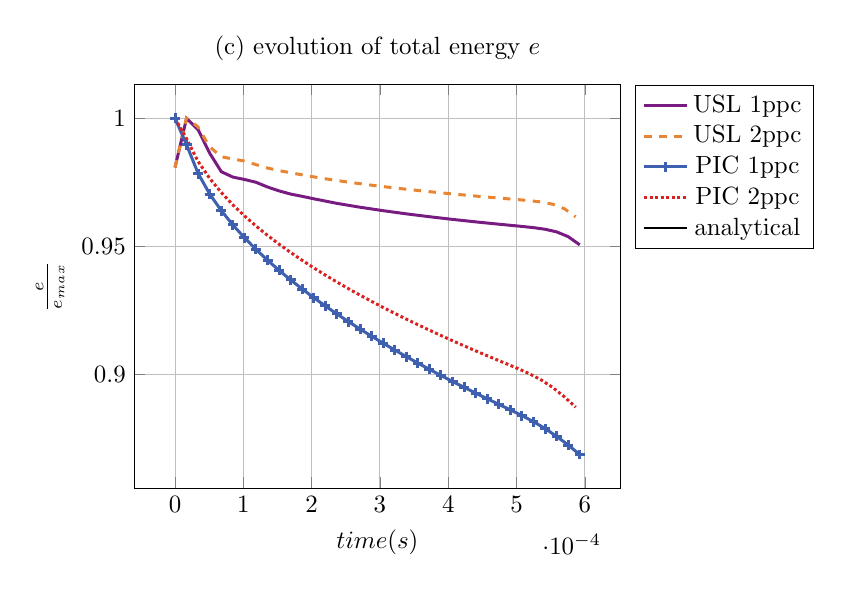
\begin{tikzpicture}[scale=0.9]
\begin{axis}[xlabel=$time (s)$,ylabel=$\frac{e}{e_{max}}$,ymajorgrids=true,xmajorgrids=true,title={(c) evolution of total energy $e$}, legend pos=outer north east]
\addplot[Purple,very thick,mark=none,solid] coordinates {(0.0,0.980776775206) (1.69272151355e-05,1.0) (3.38544302711e-05,0.995486386818) (5.07816454066e-05,0.986335480918) (6.77088605422e-05,0.979118179787) (8.46360756777e-05,0.977011836735) (0.000101563290813,0.976083552705) (0.000118490505949,0.974985958077) (0.000135417721084,0.973132007483) (0.00015234493622,0.971614043952) (0.000169272151355,0.970370597838) (0.000186199366491,0.969484052645) (0.000203126581626,0.968527091175) (0.000220053796762,0.967645365047) (0.000236981011898,0.966743210911) (0.000253908227033,0.965982183586) (0.000270835442169,0.965231974397) (0.000287762657304,0.964563191524) (0.00030468987244,0.96388114719) (0.000321617087575,0.963263530823) (0.000338544302711,0.962646353557) (0.000355471517846,0.962084695394) (0.000372398732982,0.961521764293) (0.000389325948117,0.961001071279) (0.000406253163253,0.960479919884) (0.000423180378389,0.959994795728) (0.000440107593524,0.959510651477) (0.00045703480866,0.959056403386) (0.000473962023795,0.958603029859) (0.000490889238931,0.958172736022) (0.000507816454066,0.957731808745) (0.000524743669202,0.957261239502) (0.000541670884337,0.956629022745) (0.000558598099473,0.95560284594) (0.000575525314608,0.953743784185) (0.000592452529744,0.950544066664) };
\addplot[Orange,very thick,mark=none,dashed] coordinates {(0.0,0.980776775206) (1.67562331645e-05,1.0) (3.3512466329e-05,0.996663809337) (5.02686994934e-05,0.98900666995) (6.70249326579e-05,0.985020324447) (8.37811658224e-05,0.984110580813) (0.000100537398987,0.983326915208) (0.000117293632151,0.981979184866) (0.000134049865316,0.980638155666) (0.00015080609848,0.979617302856) (0.000167562331645,0.978778886884) (0.000184318564809,0.977968446843) (0.000201074797974,0.977176694993) (0.000217831031138,0.976440965591) (0.000234587264303,0.975764557777) (0.000251343497467,0.975128766754) (0.000268099730632,0.974522184343) (0.000284855963796,0.973943735564) (0.000301612196961,0.973393220953) (0.000318368430125,0.972867749193) (0.00033512466329,0.972363947434) (0.000351880896454,0.971879647077) (0.000368637129618,0.971413467384) (0.000385393362783,0.970964070517) (0.000402149595947,0.97053007437) (0.000418905829112,0.970110254428) (0.000435662062276,0.969703595912) (0.000452418295441,0.969309210173) (0.000469174528605,0.96892621672) (0.00048593076177,0.968553101725) (0.000502686994934,0.968183689821) (0.000519443228099,0.96779053395) (0.000536199461263,0.967278784767) (0.000552955694428,0.96640240077) (0.000569711927592,0.964686590438) (0.000586468160757,0.961481917033) };
\addplot[Blue,very thick,mark=+,solid] coordinates {(0.0,1.0) (1.69272151355e-05,0.9896) (3.38544302711e-05,0.97840192) (5.07816454066e-05,0.970395814144) (6.77088605422e-05,0.963922377931) (8.46360756777e-05,0.958330092512) (0.000101563290813,0.953327939993) (0.000118490505949,0.948758714644) (0.000135417721084,0.944525461648) (0.00015234493622,0.940563061208) (0.000169272151355,0.936825160363) (0.000186199366491,0.933277336034) (0.000203126581626,0.929893178182) (0.000220053796762,0.926651891851) (0.000236981011898,0.923536752237) (0.000253908227033,0.92053406787) (0.000270835442169,0.917632461061) (0.000287762657304,0.914822354268) (0.00030468987244,0.912095594541) (0.000321617087575,0.909445173164) (0.000338544302711,0.906865012545) (0.000355471517846,0.904349801607) (0.000372398732982,0.901894866831) (0.000389325948117,0.899496069935) (0.000406253163253,0.897149725755) (0.000423180378389,0.894852535658) (0.000440107593524,0.892601494491) (0.00045703480866,0.890393110082) (0.000473962023795,0.888218874172) (0.000490889238931,0.886052220178) (0.000507816454066,0.883829497068) (0.000524743669202,0.881442958718) (0.000541670884337,0.878767030396) (0.000558598099473,0.875715616111) (0.000575525314608,0.872297097702) (0.000592452529744,0.868628627691) };
\addplot[Red,very thick,mark=none,densely dotted] coordinates {(0.0,1.0) (1.67562331645e-05,0.9921) (3.3512466329e-05,0.98321470125) (5.02686994934e-05,0.976674798128) (6.70249326579e-05,0.971199634535) (8.37811658224e-05,0.966410687731) (0.000100537398987,0.962109118378) (0.000117293632151,0.958172229577) (0.000134049865316,0.954520707917) (0.00015080609848,0.951100328411) (0.000167562331645,0.947872098186) (0.000184318564809,0.944806876372) (0.000201074797974,0.941882214857) (0.000217831031138,0.939080387869) (0.000234587264303,0.936387108509) (0.000251343497467,0.933790661554) (0.000268099730632,0.931281298637) (0.000284855963796,0.928850804847) (0.000301612196961,0.926492180888) (0.000318368430125,0.924199405234) (0.00033512466329,0.92196725296) (0.000351880896454,0.919791155586) (0.000368637129618,0.917667091102) (0.000385393362783,0.915591496621) (0.000402149595947,0.913561198187) (0.000418905829112,0.911573353815) (0.000435662062276,0.909625405615) (0.000452418295441,0.907714970883) (0.000469174528605,0.905838699657) (0.00048593076177,0.903984815557) (0.000502686994934,0.902108349787) (0.000519443228099,0.900090874846) (0.000536199461263,0.89772781162) (0.000552955694428,0.894800303924) (0.000569711927592,0.891215939989) (0.000586468160757,0.8871100207) };
\addplot[black,thick] coordinates {(0.,1.) (0.0000001,1.)};
\legend{USL 1ppc,USL 2ppc,PIC 1ppc,PIC 2ppc,analytical}
\end{axis}
\end{tikzpicture}

%%% Local Variables: 
%%% mode: latex
%%% TeX-master: "../../mainManuscript"
%%% End:
 \phantomsubcaption \label{subfig:mpm_energies}}
  \caption{MPM solutions of a bar impact problem.}
  \label{fig:mpm_diffusion}
\end{figure}
%CFL=0.7;length = 6.0;Nelem = 150;E = 2.0e11;Sigy = 400.0e7;rho = 7800.0;v0=0.5*Sigy/(2*rho*c)

Even though particles carry the whole history of the problem, FLIP has been essentialy used until the 90's to model history-independent constitutive models wich were dealt with on the grid. The first application of the method to history-dependent materials was made in the context of solid mechanics and yields the \textbf{Material Point Method} (MPM) \cite{Sulsky94}. Since this formulation was based on a weak formulation for which \textit{material points} plays the role of integration points, the MPM may be seen as an extension of the Finite Element Method with moving Gauss points. Indeed, each material point is ascribed a volume by means of a delta Dirac \textit{characteristic function} which allows to approximate the volume integrals of the weak form by discrete sums over the Lagrangian particles. However, when material points move from one cell to another, the discontinuity of the gradient of first-order shape functions yields the \textit{grid-crossing} instability \cite{Gimp}. The \textbf{Generalized Interpolation Material Point Method} (GIMP) addressed this numerical issue by modifying the particles characteristic function, thus widening the domain of influence of material points \cite{Gimp}. Although this approach enables a drastic reduction of the grid-crossing instability, it does not eliminate the oscillations in the neighborhood of discontinuous solutions (see for instance the numerical results of dynamic problems in \cite[Sec.~4.2]{Gimp}). An other way followed to tackle this issue is the direct modification of the approximation basis. In this direction, the \textbf{B-Spline Material Point Method} (BSMPM) \cite{Steffen_quadError} proposes an enrichement of the approximation basis by using quadratic or cubic B-Spline functions which provide continuous gradients and hence, the ability to circumvent the grid-crossing instability \cite{MPM_BSpline2}. Alternatively, the \textbf{Dual Domain Material Point Method} (DDMPM) \cite{DDMPM0} combined a modified gradient to classical linear shape functions so that the aforementioned instability can be eliminated as well.

+ Dire un mot sur le HighOrder MPM qui n'est pas forcément désiré car on cherche à approcher des discontinuités.


Dire qu'un champ est défini dans les cellules grâce aux fonctions de forme (notamment dans la forme faible) $q(x)=N_iq_i(x)$, ce qui sous-entend que le mapping inverse doit être fait ainsi.

We propose here an alternative way for reducing diffusion by using the DG approximation. Mapping from particles to node identical to that of MPM whil nodes to particles is the same than this of PIC but element wise due to the discontinuous approximation. Since the mapping procedure of \cite{PIC_Nishiguchi} has been identified to be responsible for oscillations \cite{Mass_Flip}

%%% Local Variables: 
%%% mode: latex
%%% TeX-master: "../mainManuscript"
%%% End:
